\section{Sensores Externos}
Los sensores externos se utilizan principalmente para saber más acerca del ambiente del robot, especialmente sobre los objetos que se va a manipular. Los sensores externos pueden
dividirse en las siguientes categorías:

\subsection{Tipo de Contacto}

\addcontentsline{toc}{subsubsection}{Interruptor de límite}
\subsection*{\quad\textbf{Interruptor de límite}}
El interruptor de límite tiene generalmente un brazo mecánico sensible a la presión. Cuando un objeto aplica presión sobre el brazo mecánico, se activa el interruptor. Es posible que un objeto tenga un imán que cause que un contacto suba y cierre cuando el objeto pase sobre el brazo. El registro de subida mantiene la señal en +V hasta que el interruptor cierra, transmitiendo la señal a tierra.\linebreak
Los interruptores de límite pueden ser normalmente abiertos (NO) o normalmente cerrados (NC) y pueden tener polos múltiples. Un interruptor normalmente abierto permite flujo de corriente hasta que se aplica presión al interruptor. 

\begin{figure}[h]
	\centering
	\subfloat[Perro]{%
		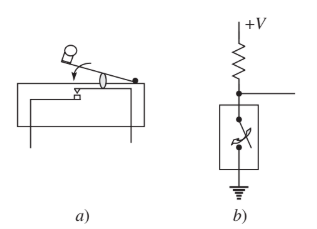
\includegraphics[width=0.2\textwidth]{Dlimite.png}%
		\label{fig:Tacómetro Comercial}
	}
	\qquad
	\subfloat[Gato]{%
		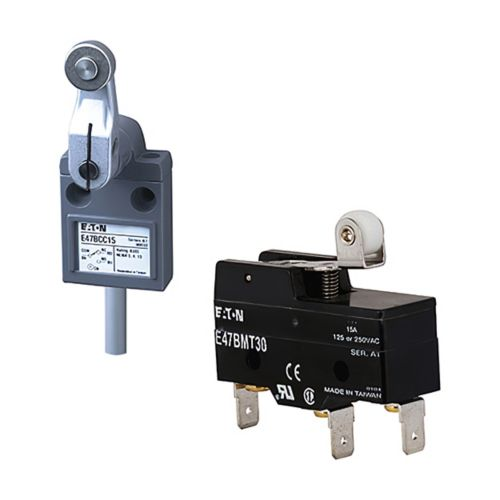
\includegraphics[width=0.2\textwidth]{Ilimite.jpg}%
		\label{fig:Diagrama Tacómetro}
	}
	\caption{Imagen de dos mascotas}
	\label{fig:Tacómetro}
\end{figure}

\addcontentsline{toc}{subsubsection}{Interruptores Neumáticos}
\subsection*{\quad\textbf{Interruptores Neumáticos}}
Los sensores neumáticos se utilizan comúnmente para la detección de desplazamiento y proximidad sin contacto, utilizando para ello instalaciones de aire comprimido. Su funcionamiento se basa en que si el aire comprimido es expulsado y no se encuentra ningún impedimento en su liberación, en las proximidades de la salida del aire al exterior no se detectará ningún aumento de presión. Sin embargo, si el aire comprimido se encuentra con algún objeto en la proximidad del orificio de salida, se podrá detectar un aumento de presión. Este aumento de presión puede ser determinado y traducido en una medida de la distancia de proximidad del objeto que obstruye la salida del aire comprimido. Los sensores neumáticos no son sensibles a señales electromagnéticas lo que les hace robustos ante interferencias de ruidos externos de este tipo. Sin embargo, para su
funcionamiento se requiere la utilización de instalaciones de aire comprimido.

\addcontentsline{toc}{subsubsection}{Sensores Piezoeléctricos}
\subsection*{\quad\textbf{Sensores Piezoeléctricos}}
Los sensores piezoeléctricos están constituidos por materiales o cristales iónicos que generan una pequeña cantidad de energía eléctrica cuando son deformados. Estos sensores son utilizados para mediciones de fuerzas y presiones aplicadas con un corto periodo de tiempo.
Cuando sobre materiales piezoeléctricos como el titanato de bario se le aplica una fuerza, las cargas negativas del material se concentran en un lado mientras que el opuesto queda cargado positivamente, generando consecuentemente un voltaje (también se producirá un cambio en Ia capacitancia).
\cite{Torres2000}

\addcontentsline{toc}{subsubsection}{Transductores de Presión}
\subsection*{\quad\textbf{Transductores de Presión}}
Un transductor de presión, a veces llamado transmisor de presión, es un transductor que convierte presión en una señal eléctrica analógica. Aunque hay varios tipos de transductores de presión, uno de los más comunes es el transductor de base de calibrador de tensión. La conversión de presión en una señal eléctrica se logra mediante la deformación física de medidores de tensión que están unidos al diafragma del transductor de presión y cableados a una configuración de puente de Wheatstone. La presión aplicada al transductor de presión produce una deflexión del diafragma que introduce tensión en los calibradores. La tensión producirá un cambio en la resistencia eléctrica proporcional a la presión. \cite{OmegaPressureTransducers}

\subsection{Tipo Sin Contacto}

\addcontentsline{toc}{subsubsection}{Sensor de Proximidad}
\subsection*{\quad\textbf{Sensor de Proximidad}}
La detección de proximidad es la técnica que se usa para detectar la presencia o ausencia de un objeto por medio de un sensor electrónico sin contacto. Hay dos tipos de sensores de proximidad: inductivo y capacitivo. Los sensores de proximidad inductivos se usan en lugar de interruptores de límite para la detección sin contacto de objetos metálicos. Los sensores de proximidad capacitivos se usan sobre la misma base que los sensores de proximidad inductivos, pero también pueden detectar objetos no metálicos.



\pagebreak
